\let\negmedspace\undefined
\let\negthickspace\undefined
\documentclass[journal,12pt,onecolumn]{article}
\usepackage{cite}
\usepackage{amsmath,amssymb,amsfonts,amsthm}
\usepackage{algorithmic}
\usepackage{graphicx}
\usepackage{textcomp}
\usepackage{xcolor}
\usepackage{txfonts}
\usepackage{listings}
\usepackage{enumitem}
\usepackage{mathtools}
\usepackage{gensymb}
\usepackage{comment}
\usepackage[breaklinks=true]{hyperref}
\usepackage{tkz-euclide} 
\usepackage{listings}
\usepackage{gvv}                                        
%\def\inputGnumericTable{}                                 
\usepackage[latin1]{inputenc}     
\usepackage{xparse}
\usepackage{color}                                            
\usepackage{array}                                            
\usepackage{longtable}                                       
\usepackage{calc}                                             
\usepackage{multirow}
\usepackage{multicol}
\usepackage{hhline}                                           
\usepackage{ifthen}                                           
\usepackage{lscape}
\usepackage{tabularx}
\usepackage{array}
\usepackage{float}
\usepackage{bm}
\newtheorem{theorem}{Theorem}[section]
\newtheorem{problem}{Problem}
\newtheorem{proposition}{Proposition}[section]
\newtheorem{lemma}{Lemma}[section]
\newtheorem{corollary}[theorem]{Corollary}
\newtheorem{example}{Example}[section]
\newtheorem{definition}[problem]{Definition}
\newcommand{\BEQA}{\begin{eqnarray}}
\newcommand{\EEQA}{\end{eqnarray}}
\usepackage{float}
%\newcommand{\define}{\stackrel{\triangle}{=}}
\theoremstyle{remark}
\usepackage{ circuitikz }
%\newtheorem{rem}{Remark}
% Marks the beginning of the document
\begin{document}

\title{CE - 2017}
\author{EE25BTECH11043 - Nishid Khandagre}
\date{}
\maketitle

\renewcommand{\thefigure}{\theenumi}
\renewcommand{\thetable}{\theenumi}

\textbf{SESSION - 1}

\begin{enumerate}
    \item The matrix $P$ is the inverse of a matrix $Q$. If $I$ denotes the identity matrix, which one of the following options is correct?\hfill (GATE-CE 2017)
    \begin{multicols}{2}
    \begin{enumerate}
        \item $PQ = I$ but $QP \neq I$
        \item $QP = I$ but $PQ \neq I$
        \item $PQ = I$ and $QP = I$
        \item $PQ - QP = I$
    \end{enumerate}
    \end{multicols}

    \item The number of parameters in the univariate exponential and Gaussian distributions, respectively, are 
    \hfill (GATE-CE 2017)
    \begin{multicols}{4}
    \begin{enumerate}
        \item 2 and 2 
        \item 1 and 2 
        \item 2 and 1 
        \item 1 and 1
    \end{enumerate}
    \end{multicols}

    \item Let $x$ be a continuous variable defined over the interval \brak{-\infty, \infty}, and f\brak{x} = e$^{{-x} - e^{-x}}$. The integral $g\brak{x}=\int f\brak{x} dx$ is equal to 
    \hfill (GATE-CE 2017)
    \begin{multicols}{2}
    \begin{enumerate}
        \item e$^{e^{-x}}$
        \item e$^{-e^{-x}}$
        \item e$^{-e^x}$
        \item e$^{-x}$
    \end{enumerate}
    \end{multicols}

    \item An elastic bar of length $L$, uniform cross sectional area $A$, coefficient of thermal expansion $\alpha$ , and Young's modulus $E$ is fixed at the two ends. The temperature of the bar is increased by $T$, resulting in an axial stress $\sigma$. Keeping all other parameters unchanged, if the length of the bar is doubled, the axial stress would be \hfill (GATE-CE 2017)
    \begin{multicols}{4}
    \begin{enumerate}
        \item $\sigma$
        \item 2$\sigma$
        \item 0.5$\sigma$
        \item 0.25 $\alpha \sigma$
    \end{enumerate}
    \end{multicols}

    \item A simply supported beam is subjected to a uniformly distributed load. \\
    Which one of the following statements is true? \hfill (GATE-CE 2017)
    \begin{enumerate}
        \item Maximum or minimum shear force occurs where the curvature is zero.
        \item Maximum or minimum bending moment occurs where the shear force is zero.
        \item Maximum or minimum bending moment occurs where the curvature is zero.
        \item Maximum bending moment and maximum shear force occur at the same section.
    \end{enumerate}

    \item According to IS 456 - 2000, which one of the following statements about the depth of neutral axis $X_{u,bal}$ for a balanced reinforced concrete section is correct? \hfill (GATE-CE 2017)
    \begin{enumerate}
        \item $X_{u,bal}$ depends on the grade of concrete only.
        \item $X_{u,bal}$ depends on the grade of steel only.
        \item $X_{u,bal}$ depends on both the grade of concrete and grade of steel.
        \item $X_{u,bal}$ does not depend on the grade of concrete and grade of steel.
    \end{enumerate}

    \item The figure shows \figref{fig:7} a two-hinged parabolic arch of span L subjected to a uniformly distributed load of intensity q per unit length.
    \begin{figure}[H]
    \centering
    \includegraphics[width=0.7\columnwidth]{figs/imageq7.jpg}  
    \caption{}
    \label{fig:7}
    \end{figure}
    The maximum bending moment in the arch is equal to \hfill (GATE-CE 2017)
    \begin{multicols}{4}
    \begin{enumerate}
        \item $\frac{qL^2}{8}$
        \item $\frac{qL^2}{12}$
        \item zero
        \item $\frac{qL^2}{10}$
    \end{enumerate}
    \end{multicols}

    \item Group I lists the type of gain or loss of strength in soils. Group II lists the property or process responsible for the loss or gain of strength in soils. \hfill (GATE-CE 2017)
    
    \begin{table}[H]
    \centering
    \begin{tabular}{|l|l|}
    \hline
    \textbf{Group-I} & \textbf{Group-II} \\
    \hline
    P. Regain of strength with time & 1. Boiling \\
    Q. Loss of strength due to cyclic loading & 2. Liquefaction \\
    R. Loss of strength due to upward seepage & 3. Thixotropy \\
    S. Loss of strength due to remolding & 4. Sensitivity \\
    \hline
    \end{tabular}
    \end{table}
    The correct match between Group I and Group II is
    \begin{enumerate}
        \item P-4, Q-1, R-2, S-3
        \item P-3, Q-1, R-2, S-4
        \item P-3, Q-2, R-1, S-4
        \item P-4, Q-2, R-1, S-3
    \end{enumerate}

    \item A soil sample is subjected to a hydrostatic pressure, $\sigma$. The Mohr circle for any point in the soil sample would be \hfill (GATE-CE 2017)
    \begin{enumerate}
        \item a circle of radius $\sigma$ and center at the origin
        \item a circle of radius $\sigma$ and center at a distance $\sigma$ from the origin
        \item a point at a distance $\sigma$ from the origin
        \item a circle of diameter $\sigma$ and center at the origin
    \end{enumerate}

    \item A strip footing is resting on the ground surface of a pure clay bed having an undrained cohesion $c_{u}$. The ultimate bearing capacity of the footing is equal to \hfill (GATE-CE 2017)
    \begin{multicols}{4}
    \begin{enumerate}
        \item $2\pi c_{u}$
        \item $\pi c_{u}$
        \item $\brak{\pi+1} c_{u}$
        \item $\brak{\pi+2} c_{u}$
    \end{enumerate}
    \end{multicols}

    \item A uniformly distributed line load of 500 kN/m is acting on the ground surface. Based on Boussinesq's theory, the ratio of vertical stress at a depth 2 m to that at 4 m, right below the line of loading, is \hfill (GATE-CE 2017)
    \begin{multicols}{4}
    \begin{enumerate}
        \item 0.25
        \item 0.5
        \item 2.0
        \item 4.0
    \end{enumerate}
    \end{multicols}

    \item For a steady incompressible laminar flow between two infinite parallel stationary plates, the shear stress variation is \hfill (GATE-CE 2017)
    \begin{enumerate}
        \item linear with zero value at the plates
        \item linear with zero value at the center
        \item quadratic with zero value at the plates
        \item quadratic with zero value at the center
    \end{enumerate}

    \item The reaction rate involving reactants A and B is given by $-k[A]^{\alpha}[B]^{\beta}$. Which one of the following statements is valid for the reaction to be a first-order reaction? \hfill (GATE-CE 2017)
    \begin{multicols}{2}
    \begin{enumerate}
        \item $\alpha = 0$ and $\beta = 0$
        \item $\alpha = 1$ and $\beta = 0$
        \item $\alpha = 1$ and $\beta = 1$
        \item $\alpha = 1$ and $\beta = 2$
    \end{enumerate}
    \end{multicols}

    \item The wastewater from a city, containing a high concentration of biodegradable organics, is being steadily discharged into a flowing river at a location S. If the rate of aeration of the river water is lower than the rate of degradation of the organics, then the dissolved oxygen of the river water \hfill (GATE-CE 2017)
    \begin{enumerate}
        \item is lowest at the location S.
        \item is lowest at a point upstream of the location S.
        \item remains constant all along the length of the river.
        \item is lowest at a point downstream of the location S.
    \end{enumerate}

    \item Which one of the following is NOT present in the acid rain? \hfill (GATE-CE 2017)
    \begin{multicols}{4}
    \begin{enumerate}
        \item HNO$_3$
        \item H$_2$SO$_4$
        \item H$_2$CO$_3$
        \item CH$_3$COOH
    \end{enumerate}
    \end{multicols}

    \item A super-elevation $e$ is provided on a circular horizontal curve such that a vehicle can be stopped on the curve without sliding. Assuming a design speed $v$ and maximum coefficient of side friction $f_{max}$, which one of the following criteria should be satisfied? \hfill (GATE-CE 2017)
    \begin{multicols}{2}
    \begin{enumerate}
        \item $e \leq f_{max}$
        \item $e > f_{max}$
        \item no limit on $e$ can be set
        \item $e = \frac{1 - (f_{max})^2}{f_{max}}$
    \end{enumerate}
    \end{multicols}

    \item A runway is being constructed in a new airport as per the International Civil Aviation Organization (ICAO) recommendations. The elevation and the airport reference temperature of this airport are 535 m above the mean sea level and 22.65$\degree$C, respectively. Consider the effective gradient of runway as 1\%. The length of runway required for a design-aircraft under the standard conditions is 2000 m. Within the framework of applying sequential corrections as per the ICAO recommendations, the length of runway corrected for the temperature is \hfill (GATE-CE 2017)
    \begin{multicols}{4}
    \begin{enumerate}
        \item 2223 m
        \item 2250 m
        \item 2500 m
        \item 2750 m
    \end{enumerate}
    \end{multicols}

    \item The accuracy of an Electronic Distance Measuring Instrument (EDMI) is specified as $\pm \brak{a mm + b ppm}$. Which one of the following statements is correct? \hfill (GATE-CE 2017)
    \begin{enumerate}
        \item Both a and b remain constant, irrespective of the distance being measured.
        \item a remains constant and b varies in proportion to the distance being measured.
        \item a varies in proportion to the distance being measured and b remains constant.
        \item Both a and b vary in proportion to the distance being measured.
    \end{enumerate}

    \item The number of spectral bands in the Enhanced Thematic Mapper sensor on the remote sensing satellite Landsat-7 is \hfill (GATE-CE 2017)
    \begin{multicols}{4}
    \begin{enumerate}
        \item 64
        \item 10
        \item 8
        \item 15
    \end{enumerate}
    \end{multicols}

    \item Consider the following partial differential equation: 
    \begin{align}
    3 \frac{\partial^2 \phi}{\partial x^2} + B \frac{\partial^2 \phi}{\partial x \partial y} + 3 \frac{\partial^2 \phi}{\partial y^2} + 4 \phi = 0
    \end{align}
    For this equation to be classified as parabolic, the value of $B^2$ must be \underline{\hspace{3cm}}\hfill (GATE-CE 2017)

    \item 
    \begin{align}
    \lim_{x \to 0} \brak{\frac{\tan x}{x^2 - x} }
    \end{align}
    is equal to \underline{\hspace{3cm}}\hfill (GATE-CE 2017)

    \item A 3 m thick clay layer is subjected to an initial uniform pore pressure of 145 kPa as shown in the figure \figref{fig:22}
    \begin{figure}[H]
    \centering
    \includegraphics[width=0.7\columnwidth]{figs/imageq22.jpg}  
    \caption{}
    \label{fig:22}
    \end{figure}
    For the given ground conditions, the time (in days, rounded to the nearest integer) required for 90\% consolidation would be \underline{\hspace{3cm}}\hfill (GATE-CE 2017)

    \item A triangular pipe network is shown in the figure \figref{fig:23}
    \begin{figure}[H]
    \centering
    \includegraphics[width=0.7\columnwidth]{figs/imageq23.jpg}  
    \caption{}
    \label{fig:23}
    \end{figure}
    The head loss in each pipe is given by $h_f = rQ^{1.8}$ , with the variables expressed in a consistent set of units. The value of $r$ for the pipe $AB$ is 1 and for the pipe $BC$ is 2. If the discharge supplied at the point $ A $ (i.e., 100) is equally divided between the pipes $AB$ and $AC$, the value of $r$ (up to two decimal places) for the pipe $AC$ should be \underline{\hspace{3cm}}\hfill (GATE-CE 2017)

    \item The ordinates of a 2-hour unit hydrograph for a catchment are given as:
    \begin{table}[H]
    \centering
    \begin{tabular}{|c|c|c|c|c|c|}
    \hline
    Time (h) & 0 & 1 & 2 & 3 & 4 \\
    \hline
    Ordinate (m$^3$/s) & 0 & 5 & 12 & 25 & 41 \\
    \hline
    \end{tabular}
    \end{table}
    The ordinate (in m$^3$/s) of a 4-hour unit hydrograph for this catchment at the time of 3 h would be \underline{\hspace{3cm}}\hfill (GATE-CE 2017)

    \item Vehicles arriving at an intersection from one of the approach roads follow the Poisson distribution. The mean rate of arrival is 900 vehicles per hour. If a gap is defined as the time difference between two successive vehicle arrivals (with vehicles assumed to be points), the probability (up to four decimal places) that the gap is greater than 8 seconds is \underline{\hspace{3cm}}\hfill (GATE-CE 2017)

    \item For the function $f\brak{x} = a + bx $, $0 \leq x \leq 1$ , to be a valid probability density function, which one of the following statements is correct? \hfill (GATE-CE 2017)
    \begin{multicols}{2}
    \begin{enumerate}
        \item a = 1, b = 4
        \item a = 0.5, b = 1
        \item a = 0, b = 1
        \item a = 1, b = -1
    \end{enumerate}
    \end{multicols}

    \item The solution of the equation $\frac{dQ}{dt} + Q = 1$ with $Q = 0$ at $t = 0$ is \hfill (GATE-CE 2017)
    \begin{multicols}{2}
    \begin{enumerate}
        \item $Q\brak{t} = e^{-t} - 1$
        \item $Q\brak{t} = 1 + e^{-t}$
        \item $Q\brak{t} = 1 - e^{t}$
        \item $Q\brak{t} = 1 - e^{-t}$
    \end{enumerate}
    \end{multicols}

    \item Consider the matrix \myvec{ 5 & -1 \\ 4 & 1 }. Which one of the following statements is TRUE for the eigenvalues and eigenvectors of this matrix? \hfill (GATE-CE 2017)
    \begin{enumerate}
        \item Eigenvalue 3 has a multiplicity of 2, and only one independent eigenvector exists.
        \item Eigenvalue 3 has a multiplicity of 2, and two independent eigenvectors exist.
        \item Eigenvalue 3 has a multiplicity of 2, and no independent eigenvector exists.
        \item Eigenvalues are 3 and -3, and two independent eigenvectors exist.
    \end{enumerate}

    \item A planar truss tower structure is shown in the figure \figref{fig:29}
    \begin{figure}[H]
    \centering
    \includegraphics[width=0.7\columnwidth]{figs/imageq29.jpg}  
    \caption{}
    \label{fig:29}
    \end{figure} 
    Consider the following statements about the external and internal determinacies of the truss:
    \begin{enumerate}
        \item Externally Determinate
        \item External Static Indeterminacy = 1
        \item External Static Indeterminacy = 2
        \item Internally Determinate
        \item Internal Static Indeterminacy = 1
        \item Internal Static Indeterminacy = 2
    \end{enumerate}
    Which one of the following options is correct? \hfill (GATE-CE 2017)
    \begin{enumerate}
        \item P-False; Q-True; R-False; S-False; T-False; U-True
        \item P-False; Q-True; R-False; S-False; T-True; U-False
        \item P-False; Q-False; R-True; S-False; T-False; U-True
        \item P-True; Q-True; R-False; S-True; T-False; U-True
    \end{enumerate}

    \item Group I contains three broad classes of irrigation supply canal outlets. Group II presents hydraulic performance attributes. The correct match of the items in Group I with the items in Group II is \hfill (GATE-CE 2017)
    
    \begin{table}[H]
    \centering
    \begin{tabular}{|l|l|}
    \hline
    \textbf{Group-I} & \textbf{Group-II} \\
    \hline
    P. Non-modular outlet & 1. Outlet discharge depends on the water levels in both the supply canal\\ & and the receiving water course\\
    Q. Semi-modular outlet & 2. Outlet discharge is fixed and is independent of the water levels \\
    R. Modular outlet & 3. Outlet discharge depends only on the water level in the supply canal \\
    \hline
    \end{tabular}
    \end{table}
    The correct match of the items in Group I and Group II
    
    \begin{enumerate}
        \item P-1; Q-2; R-3
        \item P-3; Q-1; R-2
        \item P-2; Q-3; R-1
        \item P-1; Q-3; R-2
    \end{enumerate}

    \item A 1 m wide rectangular channel has a bed slope of 0.0016 and the Manning's roughness coefficient is 0.04. Uniform flow takes place in the channel at a flow depth of 0.5 m. At a particular section, gradually varied flow (GVF) is observed and the flow depth is measured as 0.6 m. The GVF profile at that section is classified as \hfill (GATE-CE 2017)
    \begin{multicols}{4}
    \begin{enumerate}
        \item $S_1$
        \item $S_2$
        \item $M_1$
        \item $M_2$
    \end{enumerate}
    \end{multicols}

    \item The following observations are made while testing aggregate for its suitability in pavement construction:
    \begin{enumerate}
        \item Mass of oven-dry aggregate in air = 1000 g
        \item Mass of saturated surface-dry aggregate in air = 1025 g
        \item Mass of saturated surface-dry aggregate under water = 625 g
    \end{enumerate}
    Based on the above observations, the correct statement is \underline{\hspace{3cm}}\hfill (GATE-CE 2017)
    \begin{enumerate}
        \item bulk specific gravity = 2.5 and water absorption = 2.5\%
        \item bulk specific gravity = 2.5 and water absorption = 2.4\%
        \item apparent specific gravity = 2.5 and water absorption = 2.5\%
        \item apparent specific gravity = 2.5 and water absorption = 2.4\%
    \end{enumerate}

    \item The queue length (in number of vehicles) versus time (in seconds) plot for an approach to a signalized intersection with the cycle length of 96 seconds is shown in the figure \figref{fig:33}
    \begin{figure}[H]
    \centering
    \includegraphics[width=0.7\columnwidth]{figs/imageq33.jpg}  
    \caption{}
    \label{fig:33}
    \end{figure}
    At time $t = 0$, the light has just turned red. The effective green time is 36 seconds, during which vehicles discharge at the saturation flow rate, $s$ (in vph). Vehicles arrive at a uniform rate, $v$ (in vph), throughout the cycle. Which one of the following statements is TRUE?\hfill (GATE-CE 2017)
    \begin{enumerate}
        \item $v = 600 vph$,and for this cycle,the average stopped delay per vehicle = 30 sec
        \item $s = 1800 vph$,and for this cycle,the average stopped delay per vehicle = 28.125 sec
        \item $v = 600 vph$,and for this cycle,the average stopped delay per vehicle = 45 sec
        \item $s = 1200 vph$,and for this cycle,the average stopped delay per vehicle = 28.125 sec
    \end{enumerate}

    \item The radius of a horizontal circular curve on a highway is 120 m. The design speed is 60 km/hour, and the design coefficient of lateral friction between the tyre and the road surface is 0.15. The estimated value of superelevation required (if full lateral friction is assumed to develop), and the value of coefficient of friction needed (if no superelevation is provided) will, respectively, be \hfill (GATE-CE 2017)
    \begin{multicols}{2}
    \begin{enumerate}
        \item $\frac{1}{11.6}$ and 0.10
        \item $\frac{1}{10.5}$ and 0.37
        \item $\frac{1}{11.6}$ and 0.24
        \item $\frac{1}{12.9}$ and 0.24
    \end{enumerate}
    \end{multicols}

    \item The observed bearings of a traverse are given below:
    \begin{table}[H]
    \centering
    \begin{tabular}{|l|c|l|c|}
    \hline
    Line & Bearing & Line & Bearing \\
    \hline
    PQ & $46\degree15'$ & QP & $226\degree15'$ \\
    QR & $108\degree15'$ & RQ & $286\degree15'$ \\
    RS & $201\degree30'$ & SR &$20\degree30'$ \\
    ST & $321\degree45'$ & TS & $141\degree45'$ \\
    \hline
    \end{tabular}
    \end{table}
    The stations most likely to be affected by the local attraction is/are \hfill (GATE-CE 2017)
    \begin{multicols}{4}
    \begin{enumerate}
        \item Only R
        \item Only S
        \item R and S
        \item P and Q
    \end{enumerate}
    \end{multicols}

    \item The laboratory tests on a soil sample yields the following results: natural moisture content = 18\%, liquid limit = 60\%, plastic limit = 25\%, percentage of clay sized fraction = 25\%. The liquidity index and activity (as per the expression proposed by Skempton) of the soil, respectively, are \hfill (GATE-CE 2017)
    \begin{multicols}{2}
    \begin{enumerate}
        \item -0.2 and 1.4
        \item 0.2 and 1.4
        \item -1.2 and 0.714
        \item 1.2 and 0.714
    \end{enumerate}
    \end{multicols}

    \item Consider the equation $\frac{du}{dt} = 3t^2 + 1$ with $u = 0$ at $t = 0$. This is numerically solved by using the forward Euler method with a step size, $\Delta t = 2$. The absolute error in the solution at the end of the first time step is \underline{\hspace{3cm}}\hfill (GATE-CE 2017)

    \item A pre-tensioned rectangular concrete beam 150 mm wide and 300 mm depth is prestressed with three straight tendons, each having a cross-sectional area of 50 mm$^2$, to an initial stress of 1200 N/mm$^2$. The tendons are located at 100 mm from the soffit of the beam. If the modular ratio is 6, the loss of prestressing force (in kN, up to one decimal place) due to the elastic deformation of concrete only is \underline{\hspace{3cm}}\hfill (GATE-CE 2017)

    \item Consider the stepped bar made with a linear elastic material and subjected to an axial load of 1 kN, as shown in the figure \figref{fig:39}
    \begin{figure}[H]
    \centering
    \includegraphics[width=0.7\columnwidth]{figs/imageq39.jpg}  
    \caption{}
    \label{fig:39}
    \end{figure}
    Segments 1 and 2 have cross-sectional area of 100 mm$^2$ and 60mm$^2$ Young's modulus of 2$\times$10$^5$ MPa and 3$\times$10$^5$ MPa, and length of 400 mm and 900 mm. respectively. The strain energy (in N-mm, up to one decimal place) in the bar due to the axial load is \underline{\hspace{3cm}}\hfill (GATE-CE 2017)

    \item The value of M in the beam ABC shown in the figure \figref{fig:40} is such that the joint B does not rotate.
    \begin{figure}[H]
    \centering
    \includegraphics[width=0.7\columnwidth]{figs/imageq40.jpg}  
    \caption{}
    \label{fig:40}
    \end{figure}
    The value of support reaction (in kN) at B should be equal to \underline{\hspace{3cm}}\hfill (GATE-CE 2017)

    \item Consider the beam ABCD shown in the figure \figref{fig:41}
    \begin{figure}[H]
    \centering
    \includegraphics[width=0.7\columnwidth]{figs/imageq41.jpg}  
    \caption{}
    \label{fig:41}
    \end{figure}
    For a moving concentrated load of 50 kN on the beam, the magnitude of the maximum bending moment (in kN-m) obtained at the support C will be equal to \underline{\hspace{3cm}}\hfill (GATE-CE 2017)

    \item Consider two axially loaded columns, namely, 1 and 2, made of a linear elastic material with Young's modulus 2 $\times$ 10$^5$ MPa, square cross-section with side 10 mm, and length 1 m. For Column 1, one end is fixed and the other end is free. For Column 2, one end is fixed and the other end is pinned. Based on the Euler's theory, the ratio (up to one decimal place) of the buckling load of Column 2 to the buckling load of Column 1 is \underline{\hspace{3cm}}\hfill (GATE-CE 2017)

    \item A column is subjected to a load through a bracket as shown in the figure \figref{fig:43}
    \begin{figure}[H]
    \centering
    \includegraphics[width=0.7\columnwidth]{figs/imageq43.jpg}  
    \caption{}
    \label{fig:43}
    \end{figure}
    The resultant force (in kN, up to one decimal place) in the bolt 1 is \underline{\hspace{3cm}}\hfill (GATE-CE 2017)

    \item A particle of mass 2 kg is travelling at a velocity of 1.5 m/s. A force $f\brak{t} = 3t^2$ (in N) is applied to it in the direction of motion for a duration of 2 seconds, where t denotes time in seconds. The velocity (in m/s, up to one decimal place) of the particle immediately after the removal of the force is \underline{\hspace{3cm}}\hfill (GATE-CE 2017)

    \item The activity details of a project are given below:
    \begin{table}[H]
    \centering
    \begin{tabular}{|c|c|c|}
    \hline
    Activity & Depends on & Duration (in days) \\
    \hline
    P & -- & 6 \\
    Q & P & 15 \\
    R & Q, T & 12 \\
    S & R & 16 \\
    T & P & 10 \\
    U & Q, T & 14 \\
    V & U & 16 \\
    \hline
    \end{tabular}
    \end{table}
    The estimated minimum time (in days) for the completion of the project will be \underline{\hspace{3cm}}\hfill (GATE-CE 2017)

    \item It is proposed to drive H-piles up to a depth of 7 m at a construction site. The average surface area of the H-pile is 3 m$^2$ per meter length. The soil at the site is homogeneous sand, having an effective friction angle of 32$\degree$. The ground water table (GWT) is at a depth of 2 m below the ground surface. The unit weights of the soil above and below the GWT are 16 kN/m$^3$ and 19 kN/m$^3$, respectively. The total axial frictional resistance (in kN, up to one decimal place) mobilized on the pile against the driving is \underline{\hspace{3cm}}\hfill (GATE-CE 2017)

    \item The infinite sand slope shown in the figure \figref{fig:47} is on the verge of sliding failure. The ground water table coincides with the ground surface. Unit weight of water $\gamma_w$ = 9.81kN/m$^3$
    \begin{figure}[H]
    \centering
    \includegraphics[width=0.7\columnwidth]{figs/imageq47.jpg}  
    \caption{}
    \label{fig:47}
    \end{figure}
    The value of the effective angle of internal friction (in degrees, up to one decimal place) of the sand is \underline{\hspace{3cm}}\hfill (GATE-CE 2017)

    \item A sluice gate used to control the flow in a horizontal channel of unit width is shown in the figure \figref{fig:48}
    \begin{figure}[H]
    \centering
    \includegraphics[width=0.7\columnwidth]{figs/imageq48.jpg}  
    \caption{}
    \label{fig:48}
    \end{figure}
    It is observed that the depth of flow is 1.0 m upstream of the gate, while the depth is 0.2 m downstream of the gate. Assuming a smooth flow transition across the sluice gate without any energy loss, and the acceleration due to gravity as 10 m/s$^2$, the discharge (in m$^3$/s, up to two decimal places) passing under the sluice gate is \underline{\hspace{3cm}}\hfill (GATE-CE 2017)

    \item Water flows through a 90$\degree$ bend in a horizontal plane as depicted in the figure \figref{fig:49}
    \begin{figure}[H]
    \centering
    \includegraphics[width=0.7\columnwidth]{figs/imageq49.jpg}  
    \caption{}
    \label{fig:49}
    \end{figure}
    A pressure of 140 kPa is measured at Section 1-1. The inlet diameter marked at Section 1-1 is $27/\sqrt{\pi}$cm, while the nozzle diameter marked at Section 2-2 is $14/\sqrt{\pi}$cm. Assume the following:

(i) Acceleration due to gravity = 10m/s$^2$

(ii) Weights of both the bent pipe segment as well as water are negligible

(iii) Friction across the bend is negligible.

    The magnitude of the force (in kN, up to two decimal places) that would be required to hold the pipe section is \underline{\hspace{3cm}}\hfill (GATE-CE 2017)

    \item A consolidated undrained (CU) triaxial compression test is conducted on a normally consolidated clay at a confining pressure of 100 kPa. The deviator stress at failure is 80 kPa, and the pore-water pressure measured at failure is 50 kPa. The effective angle of internal friction (in degrees, up to one decimal place) of the soil is \underline{\hspace{3cm}}\hfill (GATE-CE 2017)

    \item An effective rainfall of 2-hour duration produced a flood hydrograph peak of 200 m$^3$/s. The flood hydrograph has a base flow of 20 m$^3$/s. If the spatial average rainfall in the watershed for the duration of storm is 2 cm and the average loss rate is 0.4 cm/hour, the peak of 2-hour unit hydrograph (in m$^3$/s-cm, up to one decimal place) is \underline{\hspace{3cm}}\hfill (GATE-CE 2017)

    \item The equivalent sound power level (in dB) of the four sources with the noise levels of 60 dB, 69 dB, 70 dB and 79 dB is \underline{\hspace{3cm}}\hfill (GATE-CE 2017)

    \item The spherical grit particles, having a radius of 0.01 mm and specific gravity of 3.0, need to be separated in a settling chamber.
    it is given that
    \begin{enumerate}
        \item g = 9.81 m/s$^2$
        \item the density of the liquid in the settling chamber = 1000 kg/m$^3$
        \item the kinematic viscousity of the liquid in the settling chamber = 10$^{-6}$ m$^2$/s
    \end{enumerate}
    Assuming laminar conditions, the settling velocity (in mm/s, up to one decimal place) is \underline{\hspace{3cm}}\hfill (GATE-CE 2017)

    \item Two wastewater streams A and B, having an identical ultimate BOD are getting mixed to form the stream C. The temperature of the stream A is 20$\degree$ and the temperature of the stream C is 10$\degree$. The 5-day BOD (in mg/l, up to one decimal place) of the stream C, calculated at 10$\degree$C, is \underline{\hspace{3cm}}\hfill (GATE-CE 2017)

    \item The wastewater having an organic concentration of 54 mg/l is flowing at a steady rate of 0.8 m$^3$/day through a detention tank of dimensions 2 m $\times$ 4 m $\times$ 2 m. If the contents of the tank are well mixed and the decay constant is 0.1 per day, the outlet concentration (in mg/l, up to one decimal place) is \underline{\hspace{3cm}}\hfill (GATE-CE 2017)

    \item The bacteria in milk are destroyed when it \underline{\hspace{3cm}} heated to 80$\degree$ Celsius.\hfill (GATE-CE 2017)
    \begin{multicols}{4}
    \begin{enumerate}
        \item would be
        \item will be
        \item is
        \item was
    \end{enumerate}
    \end{multicols}

    \item \underline{\hspace{3cm}} with someone else's email account is now a very serious offence.\hfill (GATE-CE 2017)
    \begin{multicols}{4}
    \begin{enumerate}
        \item Involving
        \item Assisting
        \item Tampering
        \item Incubating
    \end{enumerate}
    \end{multicols}

    \item Consider the following sentences:
    All benches are beds. No bed is a bulb. Some bulbs are lamps.
    Which of the following can be inferred? \hfill (GATE-CE 2017)

        a)Some beds are lamps.\\
        b)Some lamps are beds.
    \begin{multicols}{2}
    \begin{enumerate}
        \item only i
        \item only ii
        \item both i and ii
        \item neither i not ii
    \end{enumerate}
    \end{multicols}

    \item If the radius of a right circular cone is increased by 50\%, its volume increases by \underline{\hspace{3cm}}\hfill (GATE-CE 2017)
    \begin{multicols}{4}
    \begin{enumerate}
        \item 75\%
        \item 100\%
        \item 125\%
        \item 237.5\%
    \end{enumerate}
    \end{multicols}

    \item The following sequence of numbers is arranged in increasing order: 1, x, x, x, y, y, 9, 16, 18. Given that the mean and median are equal, and are also equal to twice the mode, the value of $y$ is 
    \hfill (GATE-CE 2017)
    \begin{multicols}{4}
    \begin{enumerate}
        \item 5
        \item 6
        \item 7
        \item 8
    \end{enumerate}
    \end{multicols}

    \item The old concert hall was demolished because of fears that the foundation would be affected by the construction of the new metro line in the area. Modern technology for underground metro construction tried to mitigate the impact of pressurized air pockets created by the excavation of large amounts of soil. But even with these safeguards, it was feared that the soil below the concert hall would not be stable.
    
    From this, one can infer that \hfill (GATE-CE 2017)
    \begin{enumerate}
        \item the foundations of old buildings create pressurized air pockets underground
        \item metro construction has to be done carefully considering its impact on existing buildings
        \item old buildings in an area form an impossible hurdle to metro construction
        \item pressurized air can be used to excavate large amounts of soil
    \end{enumerate}

    \item Students applying for hostel rooms are allotted rooms in order of seniority. Students already staying in a room will move if they get a room in their preferred list. Preferences of lower ranked applicants are ignored during allocation.
    Given the data below, which room will Ajit stay in? \hfill (GATE-CE 2017)
    \begin{table}[H]
    \centering
    \begin{tabular}{|l|c|c|l|}
    \hline
    Names & Student seniority & Current room & Room preference list \\
    \hline
    Amar & 1 & P & R, S, Q \\
    Akbar & 2 & None & R, S \\
    Anthony & 3 & Q & P \\
    Ajit & 4 & S & Q, P, R \\
    \hline
    \end{tabular}
    \end{table}
    \begin{multicols}{4}
    \begin{enumerate}
        \item P
        \item Q
        \item R
        \item S
    \end{enumerate}
    \end{multicols}

    \item The last digit of $\brak{2171}^7 + \brak{2172}^9 + \brak{2173}^{11} + \brak{2174}^{13}$ is \hfill (GATE-CE 2017)
    \begin{multicols}{4}
    \begin{enumerate}
        \item 2
        \item 4
        \item 6
        \item 8
    \end{enumerate}
    \end{multicols}

    \item Two machines M1 and M2 are able to execute any of four jobs P, Q, R and S. The machines can perform one job on one object at a time. Jobs P, Q, R and S take 30 minutes, 20 minutes, 60 minutes and 15 minutes each respectively. There are 10 objects each requiring exactly 1 job. Job P is to be performed on 2 objects, Job Q on 3 objects, Job R on 1 object and Job S on 4 objects. What is the minimum time needed to complete all the jobs? \hfill (GATE-CE 2017)
    \begin{multicols}{4}
    \begin{enumerate}
        \item 2 hours
        \item 2.5 hours
        \item 3 hours
        \item 3.5 hours
    \end{enumerate}
    \end{multicols}

    \item The bar graph below shows the output of five carpenters over one month, each of whom made different items of furniture: chairs, tables, and beds. 
    \begin{figure}[H]
    \centering
    \includegraphics[width=0.7\columnwidth]{figs/imageq65.jpg}  
    \caption{}
    \label{fig:12}
    \end{figure}
    Consider the following statements:
    \begin{enumerate}
        \item The number of beds made by carpenter C2 is exactly the same as the number of tables made by carpenter C3.
        \item The total number of chairs made by all carpenters is less than the total number of tables.
    \end{enumerate}
    Which one of the following is true? \hfill (GATE-CE 2017)
    \begin{multicols}{2}
    \begin{enumerate}
        \item Only i
        \item Only ii
        \item Both i and ii
        \item Neither i nor ii
    \end{enumerate}
    \end{multicols}
\end{enumerate}



\textbf{SESSION - 2}



\begin{enumerate}
    \item Consider the following simultaneous equations (with $c_1$ and $c_2$ being constants):
    \begin{align}
    3x_1 + 2x_2 = c_1
    \end{align}
    \begin{align}
    4x_1 + x_2 = c_2
    \end{align}
    The characteristic equation for these simultaneous equations is
    \begin{multicols}{2}
    \begin{enumerate}
        \item $\lambda^2 - 4\lambda - 5 = 0$  
        \item $\lambda^2 - 4\lambda + 5 = 0$  
        \item $\lambda^2 + 4\lambda - 5 = 0$  
        \item $\lambda^2 + 4\lambda + 5 = 0$  
    \end{enumerate}
    \end{multicols}
    \hfill (GATE-CE 2017)

    \item Let $w = f\brak{x, y}$, where $x$ and $y$ are functions of  $t$. Then, according to the chain rule, $\frac{dw}{dt}$ is equal to
    \begin{multicols}{2}
    \begin{enumerate}
        \item $\frac{dw}{dx} \frac{dx}{dt} + \frac{dw}{dy} \frac{dt}{dt} $
        \item $\frac{\partial w}{\partial x} \frac{\partial x}{\partial t} + \frac{\partial w}{\partial y} \frac{\partial y}{\partial t}$ 
        \item $\frac{\partial w}{\partial x} \frac{dx}{dt} + \frac{\partial w}{\partial y} \frac{dy}{dt}$ 
        \item $\frac{dw}{dx} \frac{\partial x}{\partial t} + \frac{dw}{dy} \frac{\partial y}{\partial t}$  
    \end{enumerate}
    \end{multicols}
    \hfill (GATE-CE 2017)

    \item Given that the scope of the construction work is well-defined with all its drawings, specifications, quantities and estimates, which one of the following types of contract would be most preferred?
    \begin{multicols}{2}
    \begin{enumerate}
        \item EPC contract  
        \item Percentage rate contract  
        \item Item rate contract  
        \item Lump sum contract  
    \end{enumerate}
    \end{multicols}
    \hfill (GATE-CE 2017)

    \item Let $G$ be the specific gravity of soil solids, $w$ the water content in the soil sample, $\gamma_w$ the unit weight of water, and $\gamma_d$ the dry unit weight of the soil. The equation for the zero air voids line in a compaction test plot is
    \begin{multicols}{4}
    \begin{enumerate}
        \item $\gamma_d = \frac{G\gamma_w}{1 + Gw}$
        \item $\gamma_d = \frac{G\gamma_w}{Gw}$
        \item $\gamma_d = \frac{Gw}{1 + \gamma_w}$ 
        \item $\gamma_d = \frac{Gw}{1 - \gamma_w}$  
    \end{enumerate}
    \end{multicols}
    \hfill (GATE-CE 2017)

    \item Consider the following statements related to the pore pressure parameters, $A$ and $B$:
    \begin{enumerate}
        \item $ A $ always lies between 0 and 1.0  
        \item $ A $ can be less than 0 or greater than 1.0  
        \item $ B $ always lies between 0 and 1.0  
        \item $ B $ can be less than 0 or greater than 1.0  
    \end{enumerate}
    For these statements, which one of the following options is correct?
    \begin{multicols}{4}
    \begin{enumerate}
        \item P and R  
        \item P and S  
        \item Q and R  
        \item Q and S  
    \end{enumerate}
    \end{multicols}
    \hfill (GATE-CE 2017)

    \item Consider a rigid retaining wall with partially submerged cohesionless backfill with a surcharge. Which one of the following diagrams closely represents the Rankine's active earth pressure distribution against this wall?
    \begin{multicols}{4}
    \begin{enumerate}
        \item (A) 
         \begin{figure}[H]
    \centering
    \includegraphics[width=0.7\columnwidth]{figs/image7a.jpg}  
    \caption{}
    \label{fig:1}
    \end{figure}
        \item (B) 
         \begin{figure}[H]
    \centering
    \includegraphics[width=0.7\columnwidth]{figs/image7b.jpg}  
    \caption{}
    \label{fig:2}
    \end{figure}
        \item (C) 
         \begin{figure}[H]
    \centering
    \includegraphics[width=0.7\columnwidth]{figs/image7c.jpg}  
    \caption{}
    \label{fig:3}
    \end{figure}
        \item (D)  
         \begin{figure}[H]
    \centering
    \includegraphics[width=0.7\columnwidth]{figs/image7d.jpg}  
    \caption{}
    \label{fig:4}
    \end{figure}
    \end{enumerate}
    \end{multicols}
   \hfill (GATE-CE 2017)

    \item If a centrifugal pump has an impeller speed of $ N $ (in rpm), discharge $ Q $ (in m$^3$/s) and the total head $ H $ (in m), the expression for the specific speed $ N_s $ of the pump is given by
    \begin{multicols}{4}
    \begin{enumerate}
        \item $ N_s = \frac{NQ^{0.5}}{H^{0.5}} $  
        \item $ N_s = \frac{NQ^{0.5}}{H} $  
        \item $ N_s = \frac{NQ^{0.5}}{H^{0.75}} $  
        \item $ N_s = \frac{NQ}{H^{0.75}} $  
    \end{enumerate}
    \end{multicols}
    \hfill (GATE-CE 2017)

    \item As per Noise Pollution (Regulation and Control) Rules 2000 of India, the day time noise limit for a residential zone, expressed in dB\brak{A} $L_{eq}$, is
    \begin{multicols}{4}
    \begin{enumerate}
        \item 55  
        \item 65  
        \item 75  
        \item 85  
    \end{enumerate}
    \end{multicols}
    \hfill (GATE-CE 2017)

    \item Following observations have been made for the elevation and temperature to ascertain the stability of the atmosphere:
    \begin{table}[H]
    \centering
    \begin{tabular}{|c|c|}
    \hline
    Elevation (in m) & Temperature (in $\degree$C) \\
    \hline
    10 & 15.5 \\
    60 & 15.0 \\
    130 & 14.3 \\
    \hline
    \end{tabular}
    \end{table}
    The atmosphere is classified as
    \begin{multicols}{4}
    \begin{enumerate}
        \item Stable  
        \item Unstable  
        \item Neutral  
        \item Inverse  
    \end{enumerate}
    \end{multicols}
    \hfill (GATE-CE 2017)

    \item The most important type of species involved in the degradation of organic matter in the case of activated sludge process is
    \begin{multicols}{2}
    \begin{enumerate}
        \item autotrophs  
        \item heterotrophs  
        \item prototrophs  
        \item photo-autotrophs  
    \end{enumerate}
    \end{multicols}
    \hfill (GATE-CE 2017)

    \item For a broad gauge railway track on a horizontal curve of radius $ R $ (in m), the equilibrium cant $ e $ required for a train moving at a speed of $ V $ (in km per hour) is
    \begin{multicols}{2}
    \begin{enumerate}
        \item $ e = 1.676 \frac{V^2}{R} $  
        \item $ e = 1.315 \frac{V^2}{R} $  
        \item $ e = 0.80 \frac{V^2}{R} $  
        \item $ e = 0.60 \frac{V^2}{R} $  
    \end{enumerate}
    \end{multicols}
    \hfill (GATE-CE 2017)

    \item The safety within a roundabout and the efficiency of a roundabout can be increased, respectively, by
    \begin{enumerate}
        \item increasing the entry radius and increasing the exit radius 
        \item increasing the entry radius and decreasing the exit radius 
        \item decreasing the entry radius and increasing the exit radius 
        \item decreasing the entry radius and decreasing the exit radius
        
    \end{enumerate}
    \hfill (GATE-CE 2017)

    \item The method of orientation used, when the plane table occupies a position not yet located on the map, is called as
    \begin{multicols}{4}
    \begin{enumerate}
        \item traversing  
        \item radiation  
        \item levelling  
        \item resection  
    \end{enumerate}
    \end{multicols}
    \hfill (GATE-CE 2017)

    \item Consider the frame shown in the figure \figref{fig:5}
    \begin{figure}[H]
    \centering
    \includegraphics[width=0.7\columnwidth]{figs/q14.jpg}  
    \caption{}
    \label{fig:5}
    \end{figure}
    If the axial and shear deformations in different members of the frame are assumed to be negligible, the reduction in the degree of kinematical indeterminacy would be equal to
    \begin{multicols}{4}
    \begin{enumerate}
        \item 5  
        \item 6  
        \item 7  
        \item 8  
    \end{enumerate}
    \end{multicols}
    \hfill (GATE-CE 2017)

    \item Let the characteristic strength be defined as that value, below which not more than 50\% of the results are expected to fall. Assuming a standard deviation of 4 MPa, the target mean strength (in MPa) to be considered in the mix design of a M25 concrete would be
    \begin{multicols}{4}
    \begin{enumerate}
        \item 18.42  
        \item 21.00  
        \item 25.00  
        \item 31.58  
    \end{enumerate}
    \end{multicols}
    \hfill (GATE-CE 2017)

    \item In a material under a state of plane strain, a $10 \times 10$\text{mm} square centered at a point gets deformed as shown in the figure \figref{fig:6}
    \begin{figure}[H]
    \centering
    \includegraphics[width=0.7\columnwidth]{figs/q16.jpg}  
    \caption{}
    \label{fig:6}
    \end{figure}
    If the shear strain $ \gamma_{xy} $ at this point is expressed as $0.001k$ (in rad), the value of $ k $ is
    \begin{multicols}{4}
    \begin{enumerate}
        \item 0.50  
        \item 0.25  
        \item -0.25  
        \item -0.50  
    \end{enumerate}
    \end{multicols}
    \hfill (GATE-CE 2017)

    \item The plate load test was conducted on a clayey strata by using a plate of $0.3m\times0.3m$ dimensions, and the ultimate load per unit area for the plate was found to be 180 kPa. The ultimate bearing capacity (in kPa) of a 2 m wide square footing would be
    \begin{multicols}{4}
    \begin{enumerate}
        \item 27  
        \item 180  
        \item 1200  
        \item 2000  
    \end{enumerate}
    \end{multicols}
    \hfill (GATE-CE 2017)

    \item For a construction project, the mean and standard deviation of the completion time are 200 days and 6.1 days, respectively. Assume normal distribution and use the value of standard normal deviate $ z = 1.64 $ for the 95\% confidence level. The maximum time required (in days) for the completion of the project would be \underline{\hspace{3cm}} \hfill (GATE-CE 2017).

    \item The divergence of the vector field $ V = x^2 i + 2 y^3 j + z^4 k $ at $ x = 1 $, $ y = 2 $, $ z = 3 $ is \underline{\hspace{3cm}} \hfill (GATE-CE 2017).

    \item A two-faced fair coin has its faces designated as head H and tail T. This coin is tossed three times in succession to record the following outcomes: H, H, H. If the coin is tossed one more time, the probability (up to one decimal place) of obtaining H again, given the previous realizations of H, H and H, would be \underline{\hspace{3cm}} \hfill (GATE-CE 2017).

    \item A sheet pile has an embedment depth of 12 m in a homogeneous soil stratum. The coefficient of permeability of soil is $10^{-6}m/s$. Difference in the water levels between the two sides of the sheet pile is 4 m. The flow net is constructed with five number of flow lines and eleven number of equipotential lines. The quantity of seepage (in cm$^3$/s per m, up to one decimal place) under the sheet pile is \underline{\hspace{3cm}} \hfill (GATE-CE 2017).

    \item The VPI (vertical point of intersection) is 100 m away (when measured along the horizontal) from the VPC (vertical point of curvature). If the vertical curve is parabolic, the length of the curve (in meters and measured along the horizontal) is \underline{\hspace{3cm}} \hfill (GATE-CE 2017).

    \item During a storm event in a certain period, the rainfall intensity is 3.5 cm/hour and the $\phi$-index is 1.5 cm/hour. The intensity of effective rainfall (in cm/hour, up to one decimal place) for this period is \underline{\hspace{3cm}} \hfill (GATE-CE 2017).

    \item The infiltration capacity of a soil follows the Horton's exponential model, $f = c_1 + c_2e^{-kt}$. During an experiment, the initial infiltration capacity was observed to be 200 mm/h. After a long time, the infiltration capacity was reduced to 25 mm/h. If the infiltration capacity after 1 hour was 90 mm/h, the value of the decay rate constant, $ k $ (in h$^{-1}$, up to two decimal places) is \underline{\hspace{3cm}} \hfill (GATE-CE 2017).

    \item While aligning a hill road with a ruling gradient of 6\%, a horizontal curve of radius 50 m is encountered. The grade compensation (in percentage, up to two decimal places) to be provided for this case would be \underline{\hspace{3cm}} \hfill (GATE-CE 2017).

    \item The tangent to the curve represented by $ y = x \ln x $ is required to have 45$\degree$ inclination with the $ x $-axis. The coordinates of the tangent point would be
    \begin{multicols}{4}
    \begin{enumerate}
        \item \brak{1,0}  
        \item \brak{0,1}  
        \item \brak{1,1}  
        \item \brak{\sqrt{2}, \sqrt{2}}  
    \end{enumerate}
    \end{multicols}
 \hfill (GATE-CE 2017)

    \item Consider the following definite integral:
    \begin{align}
    I = \int_{0}^{1} \frac{\brak{\sin^{-1} x}^2}{\sqrt{1 - x^2}} dx
    \end{align}
    The value of the integral is
    \begin{multicols}{4}
    \begin{enumerate}
        \item $\frac{\pi^3}{24}$  
        \item $\frac{\pi^3}{12}$  
        \item $\frac{\pi^3}{48}$  
        \item $\frac{\pi^3}{64}$  
    \end{enumerate}
    \end{multicols}
   \hfill (GATE-CE 2017)

    \item If $ A = \myvec{1 & 5 \\ 6 & 2} $ and $ B = \myvec{ 3 & 7 \\ 8 & 4} $, then $ AB^T $ is equal to
    \begin{multicols}{4}
    \begin{enumerate}
        \item $\myvec{ 38 & 28 \\ 32 & 56 }$  
        \item $\myvec{ 3 & 40 \\ 42 & 8 }$  
        \item $\myvec{ 43 & 27 \\ 34 & 50 }$  
        \item $\myvec{ 38 & 32 \\ 28 & 56 }$  
    \end{enumerate}
    \end{multicols}
   \hfill (GATE-CE 2017)

    \item Consider the following second-order differential equation:
    \begin{align}
    y'' - 4y' + 3y = 2t - 3t^2
    \end{align}
    The particular solution of the differential equation is
    \begin{multicols}{4}
    \begin{enumerate}
        \item $-2 - 2t - t^2$  
        \item $-2t - t^2$  
        \item $2t - 3t^2$  
        \item $-2 - 2t - 3t^2$  
    \end{enumerate}
    \end{multicols}
   \hfill (GATE-CE 2017)

    \item Group I gives a list of test methods and test apparatus for evaluating some of the properties of Ordinary Portland Cement \brak{OPC} and concrete. Group II gives the list of these properties.
    \begin{table}[H]
    \centering
    \begin{tabular}{|l|l|}
    \hline
    \textbf{Group I} & \textbf{Group II} \\
    \hline
    P. Le Chatelier test & 1. Soundness of OPC \\
    Q. Vee-Bee test & 2. Consistency and setting time of OPC \\
    R. Blaine air permeability test & 3. Consistency or workability of concrete \\
    S. The Vicat apparatus & 4. Fineness of OPC \\
    \hline
    \end{tabular}
    \end{table}
    The correct match of the items in Group I with the items in Group II is
    \begin{enumerate}
        \item P-1, Q-3, R-4, S-2  
        \item P-2, Q-3, R-1, S-4  
        \item P-4, Q-2, R-4, S-1  
        \item P-1, Q-4, R-2, S-3  
    \end{enumerate}
    \hfill (GATE-CE 2017)

    \item Two prismatic beams having the same flexural rigidity of 1000 kN-m$^2$ are shown in the figure \figref{fig:7}
    \begin{figure}[H]
    \centering
    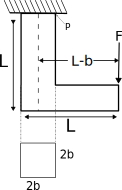
\includegraphics[width=0.7\columnwidth]{figs/q31.jpg}  
    \caption{}
    \label{fig:7}
    \end{figure}
    If the mid-span deflections of these beams are denoted by $\delta_1$ and $\delta_2$ (as indicated in the figures), the correct option is
    \begin{multicols}{4}
    \begin{enumerate}
        \item $\delta_1 = \delta_2$  
        \item $\delta_1 < \delta_2$  
        \item $\delta_1 > \delta_2$  
        \item $\delta_1 >> \delta_2$  
    \end{enumerate}
    \end{multicols}
    \hfill (GATE-CE 2017)

    \item Consider the three prismatic beams with the clamped supports $ P $, $ Q $, and $ R $ as shown in the figure \figref{fig:8}
    \begin{figure}[H]
    \centering
    \includegraphics[width=0.7\columnwidth]{figs/q32.jpg}  
    \caption{}
    \label{fig:8}
    \end{figure}
    Given that the modulus of elasticity, $ E $ is $ 2.5 \times 10^4 MPa $; and the moment of inertia, $ I $ is $ 8 \times 10^8 mm^4 $, the correct comparison of the magnitudes of the shear force $ S $ and the bending moment $ M $ developed at the supports is
    \begin{enumerate}
        \item $ S_P < S_Q < S_R $;  $ M_P = M_Q = M_R $  
        \item $ S_P = S_Q > S_R $;  $ M_P = M_Q > M_R $  
        \item $ S_P < S_Q > S_R $;  $ M_P = M_Q = M_R $  
        \item $ S_P < S_Q < S_R $;  $ M_P < M_Q < M_R $  
    \end{enumerate}
    \hfill (GATE-CE 2017)

    \item Consider the following statements:
    \begin{enumerate}
        \item P. Walls of one brick thick are measured in square meters. 
        \item Q. Walls of one brick thick are measured in cubic meters.  
        \item R. No deduction in the brickwork quantity is made for openings in walls up to 0.1 m$^2$ area.  
        \item S. For the measurement of excavation from the borrow pit in a fairly uniform ground, deadmen are left at suitable intervals.
    \end{enumerate}
    For the above statements, the correct option is
    \begin{enumerate}
        \item P - False; Q - True; R - False; S - True  
        \item P - False; Q - True; R - False; S - False  
        \item P - True; Q - False; R - True; S - False  
        \item P - True; Q - False; R - True; S - True  
    \end{enumerate}
    \hfill (GATE-CE 2017)

    \item Two identical concrete piles having the plan dimensions $ 50cm \times 50cm $ are driven into a homogeneous sandy layer as shown in the figures. Consider the bearing capacity factor $ N_q $ for $ \phi = 30\degree $ as 24.
    \begin{figure}[H]
    \centering
    \includegraphics[width=0.7\columnwidth]{figs/q34.jpg}  
    \caption{}
    \label{fig:9}
    \end{figure}
    If $ Q_{P1} $ and $ Q_{P2} $ represent the ultimate point bearing resistances of the piles under dry and submerged conditions, respectively, which one of the following statements is correct?
    \begin{enumerate}
        \item $ Q_{p1} > Q_{p2} $ by about 100\%  
        \item $ Q_{p1} < Q_{p2} $ by about 100\%  
        \item $ Q_{p1} > Q_{p2} $ by about 5\%  
        \item $ Q_{p1} < Q_{p2} $ by about 5\%  
    \end{enumerate}
    \hfill (GATE-CE 2017)

    \item Following are the statements related to the stress paths in a triaxial testing of soils:
    \begin{itemize}
        \item P. If $ \sigma_1 = \sigma_3 $, the stress point lies at the origin of the $ p-q $ plot.  
        \item Q. If $ \sigma_1 = \sigma_3 $, the stress point lies on the $ p $-axis of the $ p-q $ plot.  
        \item R. If $ \sigma_1 > \sigma_3 $, both the stress points $ p $ and $ q $ are positive.  
    \end{itemize}
    For the above statements, the correct combination is
    \begin{enumerate}
        \item P - False; Q - True; R - True  
        \item P - True; Q - False; R - True  
        \item P - False; Q - True; R - False  
        \item P - True; Q - False; R - False  
    \end{enumerate}
    \hfill (GATE-CE 2017)

    \item Two cars P and Q are moving in a racing track continuously for two hours. Assume that no other vehicles are using the track during this time. The expressions relating the distance travelled $ d $ (in km) and time $ t $ (in hour) for both the vehicles are given as
    \begin{align}
    P: d = 60t
    \end{align}
    \begin{align}
     Q: d = 60t^2
    \end{align}
    Within the first one hour, the maximum space headway would be
    \begin{multicols}{2}
    \begin{enumerate}
        \item 15 km at 30 minutes  
        \item 15 km at 15 minutes  
        \item 30 km at 30 minutes  
        \item 30 km at 15 minutes  
    \end{enumerate}
    \end{multicols}
    \hfill (GATE-CE 2017)

    \item For the construction of a highway, a cut is to be made as shown in the figure \figref{fig:9}
    \begin{figure}[H]
    \centering
    \includegraphics[width=0.7\columnwidth]{figs/q37.jpg}  
    \caption{}
    \label{fig:9}
    \end{figure}
    The soil exhibits $c' = 20 kPa$ , $\phi' = 18\degree $, and the undrained shear strength $ = 80kPa $. The unit weight of water is 9.81 kN/m$^3$. The unit weights of the soil above and below the ground water table are 18 and 20kN/m$^3$, respectively. If the shear stress at Point $ A $ is 50 kPa, the factors of safety against the shear failure at this point, considering the undrained and drained conditions, respectively, would be
    \begin{multicols}{4}
    \begin{enumerate}
        \item 1.6 and 0.9  
        \item 0.9 and 1.6  
        \item 0.6 and 1.2  
        \item 1.2 and 0.6  
    \end{enumerate}
    \end{multicols}
    \hfill (GATE-CE 2017)

    \item Two towers, A and B, standing vertically on a horizontal ground, appear in a vertical aerial photograph as shown in the figure \figref{fig:10}
    \begin{figure}[H]
    \centering
    \includegraphics[width=0.7\columnwidth]{figs/q38.jpg}  
    \caption{}
    \label{fig:10}
    \end{figure}
    The length of the image of the tower A on the photograph is 1.5 cm and of the tower B is 2.0 cm. The distance of the top of the tower A (as shown by the arrowhead) is 4.0 cm and the distance of the top of the tower B is 6.0 cm, as measured from the principal point $ p $ of the photograph. If the height of the tower B is 80 m, the height (in meters) of the tower A is \underline{\hspace{3cm}} \hfill (GATE-CE 2017).

    \item A hollow circular shaft has an outer diameter of 100 mm and inner diameter of 50 mm. If the allowable shear stress is 125 MPa, the maximum torque (in kN-m) that the shaft can resist is \underline{\hspace{3cm}} \hfill (GATE-CE 2017).

    \item A simply supported rectangular concrete beam of span 8 m has to be prestressed with a force of 1600 kN. The tendon is of parabolic profile having zero eccentricity at the supports. The beam has to carry an external uniformly distributed load of intensity 30 kN/m. Neglecting the self-weight of the beam, the maximum dip (in meters, up to two decimal places) of the tendon at the mid-span to balance the external load should be \underline{\hspace{3cm}} \hfill (GATE-CE 2017).

    \item Two plates of 8 mm thickness each are connected by a fillet weld of 6 mm thickness as shown in the figure \figref{fig:11}
    \begin{figure}[H]
    \centering
    \includegraphics[width=0.7\columnwidth]{figs/q41.jpg}  
    \caption{}
    \label{fig:11}
    \end{figure}
    The permissible stresses in the plate and the weld are 150 MPa and 110 MPa, respectively. Assuming the length of the weld shown in the figure to be the effective length, the permissible load $ P $ (in kN) is \underline{\hspace{3cm}} \hfill (GATE-CE 2017).

    \item Consider the portal frame shown in the figure \figref{fig:11} and assume the modulus of elasticity, $ E = 2.5 \times 10^4 MPa $ and the moment of inertia, $ I = 8 \times 10^8 mm^4 $ for all the members of the frame.
    \begin{figure}[H]
    \centering
    \includegraphics[width=0.7\columnwidth]{figs/q42.jpg}  
    \caption{}
    \label{fig:11}
    \end{figure}
    The rotation (in degrees, up to one decimal place) at the rigid joint Q would be \underline{\hspace{3cm}} \hfill (GATE-CE 2017).

    \item A 2 m long, axially loaded mild steel rod of 8 mm diameter exhibits the load-displacement \brak{P-\delta} behavior as shown in the figure \figref{fig:12}
    \begin{figure}[H]
    \centering
    \includegraphics[width=0.7\columnwidth]{figs/q43.jpg}  
    \caption{}
    \label{fig:12}
    \end{figure}
    Assume the yield stress of steel as 250 MPa. The complementary strain energy (in N-mm) stored in the bar up to its linear elastic behavior will be \underline{\hspace{3cm}} \hfill (GATE-CE 2017).

    \item Consider a square-shaped area $ABCD$ on the ground with its centre at $M$ as shown in the figure \figref{fig:13} . Four concentrated vertical loads of $ P = 5000 $ kN are applied on this area, one at each corner.
    \begin{figure}[H]
    \centering
    \includegraphics[width=0.7\columnwidth]{figs/q44.jpg}  
    \caption{}
    \label{fig:13}
    \end{figure}
    The vertical stress increment (in kPa, up to one decimal place) due to these loads according to the Boussinesq's equation, at a point 5 m right below $M$, is \underline{\hspace{3cm}} \hfill (GATE-CE 2017).

    \item The figure \figref{fig:13} shows a U-tube having a 5 mm $\times$ 5 mm square cross-section filled with mercury (specific gravity = 13.6) up to a height of 20 cm in each limb (open to the atmosphere).
    \begin{figure}[H]
    \centering
    \includegraphics[width=0.7\columnwidth]{figs/q45.jpg}  
    \caption{}
    \label{fig:13}
    \end{figure}
    If 5 cm$^3$ of water is added to the right limb, the new height (in cm, up to two decimal places) of mercury in the LEFT limb will be \underline{\hspace{3cm}} \hfill (GATE-CE 2017).

    \item A 1 m wide rectangular channel carries a discharge of 2 m$^3$/s. The specific energy-depth diagram is prepared for the channel. It is observed in this diagram that corresponding to a particular specific energy, the subcritical depth is twice the supercritical depth. The subcritical depth (in meters, up to two decimal places) is equal to \underline{\hspace{3cm}} \hfill (GATE-CE 2017).

    \item A catchment is idealized as a 25 km $\times$ 25 km square. It has five rain gauges, one at each corner and one at the center, as shown in the figure  \figref{fig:14}
    \begin{figure}[H]
    \centering
    \includegraphics[width=0.7\columnwidth]{figs/q47.jpg}  
    \caption{}
    \label{fig:14}
    \end{figure}
    During a month, the precipitation at these gauges is measured as $ G_1 = 300 mm $, $ G_2 = 285mm $, $ G_3 = 272mm $, $ G_4 = 290mm $ and $ G_5 = 288mm $. The average precipitation (in mm, up to one decimal place) over the catchment during this month by using the Thiessen polygon method is \underline{\hspace{3cm}} \hfill (GATE-CE 2017).

    \item The culturable command area of a canal is 10,000 ha. The area grows only two crops-rice in the Kharif season and wheat in the Rabi season. The design discharge of the canal is based on the rice requirements, which has an irrigated area of 2500 ha, base period of 150 days and delta of 130 cm. The maximum permissible irrigated area (in ha) for wheat, with a base period of 120 days and delta of 50 cm, is \underline{\hspace{3cm}} \hfill (GATE-CE 2017).

    \item Water is pumped at a steady uniform flow rate of 0.01 m$^3$/s through a horizontal smooth circular pipe of 100 mm diameter. Given that the Reynolds number is 800 and $ g $ is 9.81 m/s$^2$, the head loss (in meters, up to one decimal place) per km length due to friction would be \underline{\hspace{3cm}} \hfill (GATE-CE 2017).

    \item The composition of a municipal solid waste sample is given below:
    \begin{table}[H]
    \centering
    \begin{tabular}{|l|c|c|c|}
    \hline
    \textbf{Component} & \textbf{Percent by Mass} & \textbf{Moisture Content (\%)} & \textbf{Energy Content (kJ/kg, on} \\ & & &  \textbf{as-discarded basis)} \\
    \hline
    Food Waste & 20 & 70 & 2500 \\
    Paper & 10 & 4 & 10000 \\
    Cardboard & 10 & 4 & 8000 \\
    Plastics & 10 & 1 & 14000 \\
    Garden Trimmings & 40 & 60 & 3500 \\
    Wood & 5 & 20 & 14000 \\
    Tin Cans & 5 & 2 & 100 \\
    \hline
    \end{tabular}
    \end{table}
    The difference between the energy content of the waste sample calculated on dry basis and as-discarded basis (in kJ/kg) would be \underline{\hspace{3cm}} \hfill (GATE-CE 2017).

    \item For a given water sample, the ratio between $BOD_{5-day,20\degree C}$ and the ultimate BOD is 0.68. The value of the reaction rate constant $ k $ (on base $ e $) (in day$^{-1}$, up to two decimal places) is \underline{\hspace{3cm}} \hfill (GATE-CE 2017).

    \item A municipal corporation is required to treat 1000 m$^3$/day of water. It is found that an overflow rate of 20 m/day will produce a satisfactory removal of the discrete suspended particles at a depth of 3 m. The diameter (in meters, rounded to the nearest integer) of a circular settling tank designed for the removal of these particles would be \underline{\hspace{3cm}} \hfill (GATE-CE 2017).

    \item The analysis of a water sample produces the following results:
    \begin{table}[H]
    \centering
    \begin{tabular}{|l|c|c|}
    \hline
    \textbf{Ion} & \textbf{milligram per milli-equivalent for the ion} & \textbf{Concentration (mg/L)} \\
    \hline
    Ca$^{2+}$ & 20.0 & 60 \\
    Mg$^{2+}$ & 12.2 & 36.6 \\
    Na$^{+}$ & 23.0 & 92 \\
    K$^{+}$ & 39.1 & 78.2 \\
    Cl$^{-}$ & 35.5 & 71 \\
    SO$_{4}^{2-}$ & 48.0 & 72 \\
    HCO$_{3}^{-}$ & 61.0 & 122 \\
    \hline
    \end{tabular}
    \end{table}
    The total hardness (in mg/L as CaCO$_{3}$) of the water sample is \underline{\hspace{3cm}} \hfill (GATE-CE 2017).

    \item The radii of relative stiffness of the rigid pavements P and Q are denoted by $l_p$ and $l_q$, respectively. The geometric and material properties of the concrete slab and underlying soil are given below:
    \begin{table}[H]
    \centering
    \begin{tabular}{|l|c|c|c|c|c|c|}
    \hline
    \textbf{Pavement} & \textbf{Length of} & \textbf{Breadth} & \textbf{Thickness} & \textbf{Modulus of} & \textbf{Poisson's} & \textbf{Subgrade} \\
    & \textbf{Slab} & \textbf{of Slab} & \textbf{of Slab} & \textbf{Elasticity} & \textbf{Ratio} & \textbf{Reaction} \\
    & & & & & & \textbf{Modulus} \\
    \hline
    P & L & B & h & E & $\micro$ & K \\
    Q & L & B & 0.5h & E & $\micro$ & 2K \\
    \hline
    \end{tabular}
    \end{table}
    The ratio (up to one decimal place) of $ l_p / l_q $ is \underline{\hspace{3cm}} \hfill (GATE-CE 2017).

    \item An observer standing on the deck of a ship just sees the top of a lighthouse. The top of the lighthouse is 40 m above the sea level and the height of the observer's eye is 5 m above the sea level. The distance (in km, up to one decimal place) of the observer from the lighthouse is \underline{\hspace{3cm}} \hfill (GATE-CE 2017).

    \item The event would have been successful if you \underline{\hspace{3cm}} able to come.
    \begin{multicols}{2}
    \begin{enumerate}
        \item are  
        \item had been  
        \item have been  
        \item would have been  
    \end{enumerate}
    \end{multicols}
    \hfill (GATE-CE 2017)

    \item There was no doubt that their work was \underline{thorough}.
    
    Which of the words below is closest in meaning to the underline word above? 
    \begin{multicols}{4}
    \begin{enumerate}
        \item pretty  
        \item complete  
        \item sloppy  
        \item haphazard  
    \end{enumerate}
    \end{multicols}
   \hfill (GATE-CE 2017)

    \item Four cards lie on a table. Each card has a number printed on one side and a colour on the other. The faces visible on the cards are 2, 3, red, and blue.
    
    Proposition: If a card has an even value on one side, then its opposite face is red.
    
    The card which MUST be turned over to verify the above proposition are
    \begin{multicols}{4}
    \begin{enumerate}
        \item 2, red  
        \item 2, 3, red  
        \item 2, blue  
        \item 2, red, blue  
    \end{enumerate}
    \end{multicols}
    \hfill (GATE-CE 2017)

    \item What is the value of $ x $ when $ 81 \times \brak{\frac{16}{25}}^{x+2} \div \brak{\frac{3}{5}}^{2x+4} = 144 $?
    \begin{multicols}{2}
    \begin{enumerate}
        \item 1  
        \item -1  
        \item -2  
        \item Cannot be determined  
    \end{enumerate}
    \end{multicols}
    \hfill (GATE-CE 2017)

    \item Two dice are thrown simultaneously. The probability that the product of the numbers appearing on the top faces of the dice is a perfect square is
    \begin{multicols}{4}
    \begin{enumerate}
        \item 1/9  
        \item 2/9  
        \item 1/3  
        \item 4/9  
    \end{enumerate}
    \end{multicols}
   \hfill (GATE-CE 2017)

    \item Bhaichung was observing the pattern of people entering and leaving a car service centre. There was a single window where customers were being served. He saw that people inevitably came out of the centre in the order that they went in. However, the time they spent inside seemed to vary a lot: some people came out in a matter of minutes while for others it took much longer.
    
    From this what can one conclude?
    \begin{enumerate}
        \item The centre operates on a first-come-first-served basis, but with variable service times, depending on specific customer needs.  
        \item Customers were served in an arbitrary order, since they took varying amounts of time for service completion in the centre.  
        \item Since some people came out within a few minutes of entering the centre, the system is likely to operate on a last-come-first-served basis.  
        \item Entering the centre early ensured that one would have shorter service times and most people attempted to do this.  
    \end{enumerate}
    \hfill (GATE-CE 2017)

    \item A map shows the elevations of Darjeeling, Gangtok, Kalimpong, Pelling, and Siliguri.  
    Kalimpong is at a lower elevation than Gangtok. Pelling is at a lower elevation than Gangtok.  
    Pelling is at a higher elevation than Siliguri. Darjeeling is at a higher elevation than Gangtok.

    Which of the following statements can be inferred from the paragraph above?
    \begin{itemize}
    \item i) Pelling is at a higher elevation than Kalimpong 
    \item ii) Kalimpong is at a lower elevation than Darjeeling 
    \item iii) Kalimpong is at a higher elevation than Silguri 
    \item iv) Silguri is at a lower elevation than Gangtok
    \end{itemize}
    
    \begin{multicols}{2}
    \begin{enumerate}
        \item Only ii  
        \item Only ii and iii  
        \item Only ii and iv  
        \item Only iii and iv  
    \end{enumerate}
    \end{multicols}
   \hfill (GATE-CE 2017)

    \item P, Q, R, S, T and U are seated around a circular table. R is seated two places to the right of Q. P is seated three places to the left of R. S is seated opposite U. If P and U now switch seats, which of the following must necessarily be true?
    \begin{enumerate}
        \item P is immediately to the right of R  
        \item T is immediately to the left of P  
        \item T is immediately to the left of P or P is immediately to the right of Q  
        \item U is immediately to the right of R or P is immediately to the left of T  
    \end{enumerate}
    \hfill (GATE-CE 2017)

    \item Budhan covers a distance of 19 km in 2 hours by cycling one fourth of the time and walking the rest. The next day he cycles (at the same speed as before) for half the time and walks the rest (at the same speed as before) and covers 26 km in 2 hours. The speed in km/h at which Budhan walks is
    \begin{multicols}{4}
    \begin{enumerate}
        \item 1  
        \item 4  
        \item 5  
        \item 6  
    \end{enumerate}
    \end{multicols}
    \hfill (GATE-CE 2017)

    \item The points in the graph \figref{fig:14} below represent the halts of a lift for durations of 1 minute, over a period of 1 hour.
    \begin{figure}[H]
    \centering
    \includegraphics[width=0.7\columnwidth]{figs/q65.jpg}  
    \caption{}
    \label{fig:14}
    \end{figure}
    Which of the following statements are correct?
    \begin{itemize}
        \item The elevator never moves directly from any non-ground floor to another non-ground floor over the one hour period  
        \item The elevator stays on the fourth floor for the longest duration over the one hour period  
    \end{itemize}
    \begin{multicols}{2}
    \begin{enumerate}
        \item only i
        \item only ii
        \item both i and ii
        \item neither i nor ii
    \end{enumerate}
    \end{multicols}
    \hfill (GATE-CE 2017)

\end{enumerate}
\end{document}

